\label{organ}
%insert organization, schedule and cost estimates here

\subsection{Schedule}
The major milestones for the proposed CERN prototype detector construction and beam test is dictated by the DUNE overall schedule which foresees to place the first 10~kton detector module underground as early as calendar year 2021. Additional detector modules, possibly of different design, are expected to follow at intervals of 1-2 years in a technically driven schedule.
Information and experience gained from manufacturing, installing and operating the CERN detector test will inform decision regarding future DUNE far detectors.
The LHC long shutdown, which is presently scheduled for mid-2018 represents a significant constraint on the beam data run schedule.
Cosmic muon data taking and ideally also beam data taking for the proposed measurement program 
should be acquired prior to  the long LHC shutdown in mid-2018. 
While it is desirable to have results from the charged particle beam run available as soon as possible the value of these results is not diminished if they become available only after installation of the DUNE far detector.
Figure \ref{fig:schedule} shows a technically limited schedule which meets the above requirements.
%is based on experiences from the production and installation schedule for the 35~t detector.
This schedule is based on experience of designing and manufacturing components for the 35t detector which will be commissioned starting in August 2015 at  Fermilab.
%
\begin{figure}[htb]
  \centering
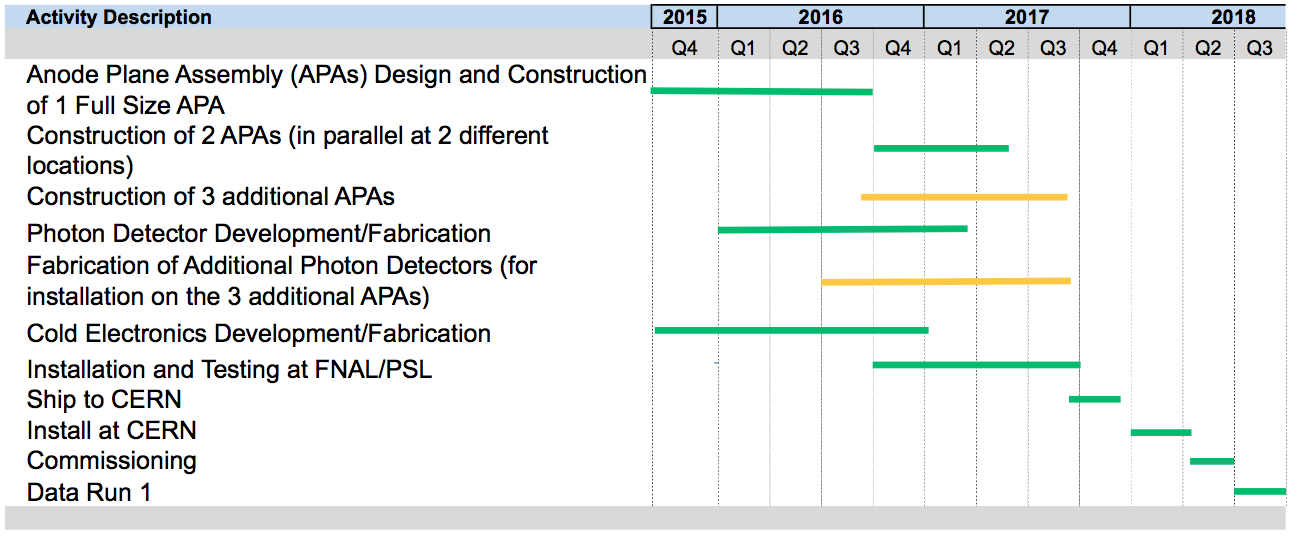
\includegraphics[scale=0.34]{figures/150514_CERN_test_sched.png}
  \caption{Rolled up version of a draft schedule for manufacturing, installing and commissioning the CERN prototype detector. A 2 - 3 months data taking period is included in the schedule. }
  \label{fig:schedule}
\end{figure}
%
Pending an approval of the effort proposed in this document we foresee the following milestones
\begin{itemize}
\item 2016: Cryostat constructed
\item early 2016: TPC production readiness review
\item spring 2017: Engineering Trial Detector Assembly
\item early 2018: Detector Installation
\item spring 2018: Detector commissioning 
\end{itemize}


\subsection{Organization}

The CERN single phase detector effort is an integral part of the DUNE collaboration and the DUNE project structure. 
A working group has been set up within the DUNE collaboration to coordinate all aspects relevant for the CERN single phase prototype detector and beam test. 

The CERN prototype effort is coordinated by the "CERN Prototype Technical Coordinator (CTC)" \cite{LBNEorg}.
%The charge of the CERN prototype Collaboration Technical Coordinator is defined as follows.
The CERN prototype CTC is responsible for the following:
\begin{enumerate}[i]
	\item Prioritize and maintain a schedule of collaboration activities regarding simulations and physics analysis. 
	\item Prioritize and maintain a schedule of other collaboration service activities on the CERN prototype.  These activities may include collaboration participation in assembly, commissioning, calibration, debugging, data-taking, shifts, etc. 
	\item The responsibility of the CERN prototype CTC shall include maintaining a database of contributions from the collaboration to the CERN detector and beam test prototyping.
	\item The CERN prototype CTC shall recruit collaboration personnel and resources.
	\item The CERN prototype CTC shall coordinate with the DUNE far detector L-2 project manager and the DUNE technical coordinator
\end{enumerate}
There are currently one CTC,Thomas Kutter (LSU)  and a deputy, Greg Pawloski (Minnesota) sharing the responsibilities.\\
 

In order to effectively execute the tasks required for the CERN prototype detector and beam test several sub-groups have been created 
and sub-group leaders have been appointed.

{\bf Measurement Program + Analysis :}   Their charge is to develop a comprehensive and prioritized list of measurements required to evaluate detector performance and provide detector charged particle response as input into DUNE physics sensitivity studies (beam physics, nucleon decay, supernovae, atmospheric neutrinos).  And to perform simulation studies to quantitatively compare the relevance of various measurements.
The leaders are Donna Naples (Pittsburgh) and Jaroslaw Nowak (Lancaster).
 
 
{\bf Beam :} Their charge is to work closely with the measurement group to identify ideal beam requirements, to work closely with the CERN beam group to develop realistic beam design to make relevant beam measurements, to evaluate and optimize possible beam injection points and beam orientations, to perform beam simulations and provide simulated beam spectra as input for detector response simulations, to identify required beam instrumentation for beam characterization, and to develop beam run plans.
The  beam subgroup leader is Cheng-Ju Lin (LBNL).


{\bf Calibration :}  Their charge is to develop tools to calibrate the performance of the detector, to interface with the physics measurement group to prioritize different calibration measurements, and to interface with detector subcomponent working groups to identify all required calibration tools and their integration into the detector /cryostat design.
The calibration sub-group leaders are Qiuguang Liu (LANL) [interim] and Michele Weber (Bern).\\


The CERN prototype coordinators work closely with the DUNE technical coordinator and the DUNE far detector manager.
%Direct communication with  DUNE spokespeople is important for any strategic issues.
The CTC also coordinates closely with the CERN Neutrino Platform leader.
The leaders of the "measurement program + analysis" subgroup work closely with the DUNE physics and software tools working group leaders. The leader of the "beam" subgroup works closely with the relevant CERN beam-line group leader.

The project work break down structure (WBS) for the CERN single phase prototype detector down to level 3 and along with contributing institutions is shown in table~\ref{tab:wbs}.
%
\begin{table}[h]
\centering
\begin{tabular}{|l l c|}
\hline
\textbf{WBS no. } & \textbf{Description}  & \textbf{Contributing Institutes}  \\ \hline

X.1 & Single Phase LAr detector & \\
X.1.1 & TPC & Wisconsin \\
X.1.2 & Photon Detection System  &  ANL, CSU, IU, LSU \\
X.1.3 & Electronics  &   \\
X.1.4 &  DAQ & Oxford, SLAC  \\
X.1.5 & Installation  & Duke  \\
X.1.6 & ...  & ...  \\ \hline

X.2 & Experiment Infrastructure  &   \\
X.2.1 & Cryostat + Top Cap &  CERN, Fermilab \\
X.2.2 & Cryogenics System  &  CERN, Fermilab \\
X.2.3 &  Slow control ? &  CERN \\
X.2.4 &  Clean Room & CERN   \\ 
X.2.5 &  Logistics \& Integration & CERN  \\ 
X.2.6 &  Detector Commissioning \& operations &  all  \\ 
X.2.7 &  Beam \& Run Coordination &  LBNL, CERN \\ \hline

X.3 &  Safety ?? &   \\ \hline

X.4 & Scientific Effort &    \\ 
X.4.1 & Software \& Simulations &  all  \\
X.4.2 & Data analysis &  all  \\ \hline

\end{tabular}
\caption{Work break down structure down to level 3.}
\label{tab:wbs}
\end{table}
%
Work on a MOU between the CERN nu-platform and DUNE describing responsibilities, listing institutions involved and defining deliverables has started. 
%

\subsection{Cost estimate}
The total estimated cost of the CERN single phase LAr prototype detector is presented in table~\ref{tab:cost}.
Cost figures are informed by component production for the 35~t detector.

\begin{table}[h!]
\centering
\begin{tabular}{| l| l| c |}
\hline
\textbf{no. } & \textbf{Item}  & \textbf{Cost [k USD]}  \\ \hline
1 & APAs & \\
2 & CPA  & \\
3 &PDS  & \\
4 & & \\
5 & & \\
7 & & \\
8 & & \\ \hline
  & \textbf{Total } & \\ \hline
\end{tabular}
\caption{Detector component cost estimate.}
\label{tab:cost}
\end{table}

%\subsection{Division of Responsibilities}


%\subsubsection{Shared responsibilities}

%The engineering design of the cryostat and the cryogenics system is considered to be a shared responsibility between DUNE/LBNF and CERN.


%\begin{itemize}

%\item plans for data analysis and publications:\\
%include: description of overlap/commonalities with WA105 data analysis and joined efforts
%\end{itemize}




%\subsubsection{CERN responsibilities}

%\paragraph{The beam line:} design, setup of the beam line and beam monitoring instrumentation are expected to be provided by CERN.

%\paragraph{The cryostat and cryogenics system:} are expected to be organized and paid for by the CERN nu-platform.
%The scope of the EHN1 cryostat subsystem includes the design, procurement, fabrication, testing, delivery and oversight of a cryostat to contain the liquid argon and the TPC.\\

%\paragraph{DAQ requests:}  Data links of sufficient bandwidth to transfer the data files from the CENF to the CERN data center, and from there to locations worldwide for analysis. \\

%\paragraph{Computing/Software support:} In order to leverage existing software and expertise, appropriate manpower will need to be allocated in order to create and maintain the computing infrastructure necessary for effective use of the reconstruction and physics analysis tools.\\



